\chapter{Load-Flow Calculation}

To clarify the situation I will start with the problem formulation in \secref{problem_formulation}. Afterwards, I will go more into detail of the certain steps which are necessary to model a power net in \secref{scaling} and \secref{modelling}. The final part of this chapter is then the description of the implemented calculation methods \secref{calculation_methods}. To be able to compare the iterative methods with \emph{HELM} I implemented them too, therefore I included these derivations and formulas in the last section too.

\section{Problem Formulation}
\label{sec:problem_formulation}

The aim of a load-flow analysis is to determine the voltages in the power net. Any further information, like currents in connections, critically low voltages, etc. can be derived from these voltages. Therefore, I will consider the problem as solved if the voltages are known.

The first step in a load-flow analysis is the modelling of the net elements, as it is way to complex to use a detailed description of for instance a power plant like \figref{power_plant}. Therefore, all elements in a power net are modelled through busses, also called nodes, and admittances between them. To simplify the calculations only single phase nets are considered. Consequently, three phase systems have to be scaled down by the factor 3, respective $\sqrt{3}$, to be represented by a single phase system. Asymmetric cases can be modelled with only single phase nets through symmetrical components \citep[p. 399]{powerSystemAnalysis}. Besides that, in the final model also exists only one voltage level, which means that all admittances, powers and voltages have to be scaled down to this voltage level.

The second step is then the actual calculation of the node voltages, which is based on a nodal analysis. As a pure nodal analysis is only capable of current loads it is extended to support more realistic load models, which define for instance the power at a node.

\begin{figure}
	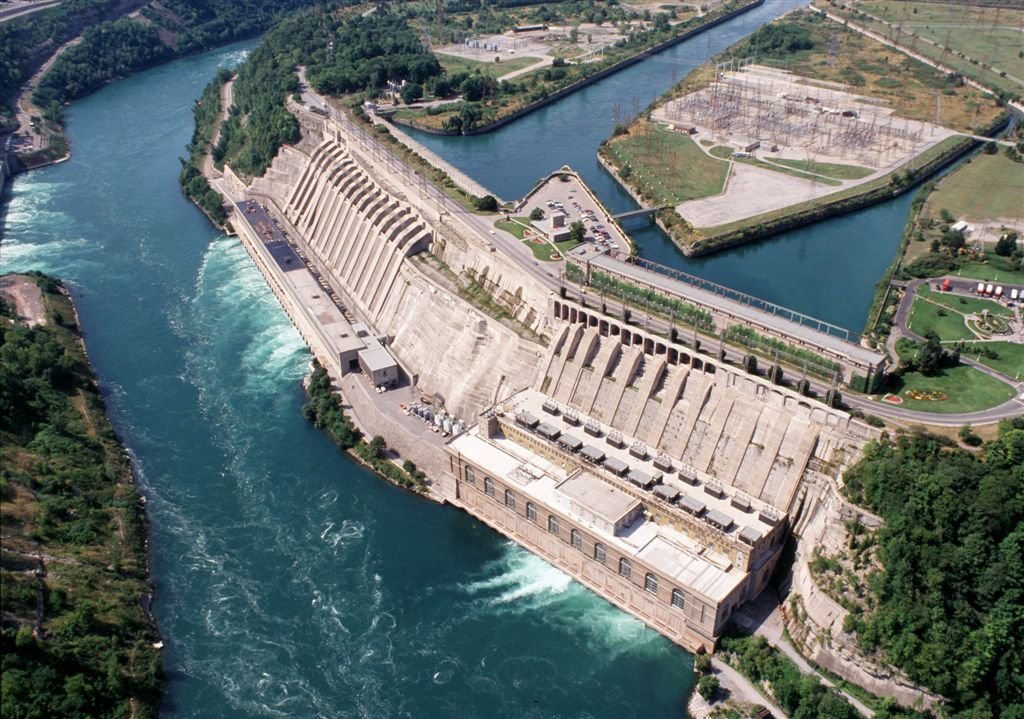
\includegraphics[width=\textwidth]{figures/adam_beck_complex.jpg}
	\caption{Sir Adam Beck Hydroelectric Generating Stations \citep{adam_back_complex}}
	\label{fig:power_plant}
\end{figure}

\subsection{Busses}

The most basic mathematical description of an electric circuit, which a power net is, would be through admittances $Y_{ki}$ between the nodes $k$ and $i$, node voltages $U_k$ and branch currents $I_k$. In this case we will use the element-based version
\begin{equation}
	\sum_i Y_{ki} U_i = I_k,
	\label{eq:current_controlled}
\end{equation}
of
\begin{equation}
	\mat Y \vec U = \vec I,
\end{equation}
as in the end the right hand side of this equation can not be described with a vector notation.

If the loads and inputs would be current-controlled we could already stop at this point, solve the equation system and receive the node voltages as the result. Unfortunately, most elements in a power net are defined through power, which is fed in, or load, which is drawn from the power net. Therefore, we have to extend \eqref{current_controlled} with a term for a constant power $S_k = P_k + j Q_k = U_k I_k^\star$ at the node $k$ and receive
\begin{equation}
	\sum_i Y_{ki} U_i = I_k + \frac{S_k^\star}{U_k^\star},
	\label{eq:pq_bus}
\end{equation}
which is already the definition of a PQ-bus. As a short side remark, a positive power means in this formulation that power is drawn from the net. Consequently, real loads are modelled with a negative sign and generators with a positive one.

Another possible type of bus is a slack bus. At this bus the voltage is defined, therefore we do not need to add a line to the equation system, but the bus is also part from neighbour busses through the branch currents $Y_{ki} U_i$. We can represent all these known branch currents on the right hand side of \eqref{pq_bus} through
\begin{equation}
	I_k = -\sum_{\text{slack busses}} Y_{ki} U_i.
\end{equation}
Although, slack busses show up only in the constant currents of the right hand side, there must be always at least one slack bus in the power net, as this bus then defines the rotation of the system and compensates mismatches in the total power sum. In practice, typically a major power plant is selected as slack bus.

The third important type of bus, besides the slack bus and PQ-bus, is the PV-bus. This is already some sort of control, as at such a node the real power $P_k$ and the voltage magnitude $|U_k|$ is defined. The implementation of this bus type depends on the algorithm which is used to calculate the missing node voltages, therefore I will discuss this in the section about the algorithms.

\subsection{Admittance Matrix}

The admittance matrix $\mat Y = (Y_{ki})$ is filled with the admittances between the nodes. More complex elements, like controlled sources, have to be represented by an equivalent circuit which is voltage controlled, so that they can be modelled with an admittance matrix. Not voltage controlled can be transformed through a gyrator, which itself can be modelled through voltage controlled elements.

As during the modelling later several kinds of electric elements will be used I will describe for each of them how they effect the admittance matrix. Each circuit element is there defined through a partial admittance matrix $\mat Y_p$. These partial matrices have to be summed up afterwards to get the total admittance matrix $\mat Y$:
\begin{equation}
	\mat Y = \sum_i \mat Y_{p,i}
\end{equation}

The same superposition applies also for the current sources, if there are any.
\begin{equation}
	\vec I = \sum_i \vec I_{p,i}
\end{equation}

The two most important elements are the admittance, which is part of nearly every model of a net element, and the ideal transformer, which is mainly used for modelling real transformers with non-nominal ratios. The controlled source and the gyrator are actually only used to model the ideal transformer.

\subsubsection{Admittance}

\begin{figure}
	\centering
	\begin{circuitikz}
	\draw (0, 0) node[left] {$U_\alpha$} to [R=$G$,o-o] (3, 0) node[right] {$U_\beta$};
\end{circuitikz} 

	\caption{Admittance $G$ between the nodes $\alpha$ and $\beta$}
	\label{fig:admittance}
\end{figure}

The admittance $G$ between the nodes $\alpha$ and $\beta$ \figref{admittance} causes the currents
\begin{equation}
	I_\alpha = (U_{k,\alpha} - U_{k,\beta}) G
\end{equation}
and
\begin{equation}
	I_\beta = (U_{k,\beta} - U_{k,\alpha}) G,
\end{equation}
which have to be considered in the admittance matrix through
\begin{equation}
	\mat Y_p = 	
	\begin{blockarray}{cccccc}
		\begin{block}{[ccccc]c}
		 		& \vdots	&			& \vdots	&			& \\
		\cdots	& G			& \cdots	& -G		& \cdots	& \alpha \\
		 		& \vdots	&			& \vdots	&			& \\
		\cdots	& -G		& \cdots	& G			& \cdots	& \beta \\
		 		& \vdots	&			& \vdots	&			& \\
		\end{block}
				& \alpha	&			& \beta		&			& 
	\end{blockarray}
\end{equation}

\subsubsection{Voltage Controlled Current Source}

\begin{figure}
	\centering
	\begin{circuitikz}
	\draw (0, 0) node[left] {$U_\delta$} to[open,o-o,v^=$u_{in}$] (0, 4) node[left] {$U_\gamma$};
	\draw (3, 4) to[european controlled current source,i=$g_m u_{in}$] (3, 0);
	\draw (3, 4) to[short,-o] (4, 4) node[right] {$U_\alpha$};
	\draw (3, 0) to[short,-o] (4, 0) node[right] {$U_\beta$};
\end{circuitikz} 

	\caption{Voltage controlled current source}
	\label{fig:voltage_controlled_current_source}
\end{figure}

The voltage controlled current source (VCCS) is defined through the two branch currents
\begin{equation}
	I_\alpha = (U_{k,\gamma} - U_{k,\delta}) g_m
\end{equation}
and
\begin{equation}
	I_\beta = (U_{k,\delta} - U_{k,\gamma}) g_m.
\end{equation}

The difference to the admittance matrix is that this time the current is controlled by different nodes, what results in the asymmetric admittance matrix
\begin{equation}
	\mat Y_p = 	
	\begin{blockarray}{cccccc}
		\begin{block}{[ccccc]c}
		 		& \vdots	&			& \vdots	&			& \\
		\cdots	& g_m		& \cdots	& -g_m		& \cdots	& \alpha \\
		 		& \vdots	&			& \vdots	&			& \\
		\cdots	& -g_m		& \cdots	& g_m		& \cdots	& \beta \\
		 		& \vdots	&			& \vdots	&			& \\
		\end{block}
				& \gamma	&			& \delta	&			& 
	\end{blockarray}.
\end{equation}

\subsubsection{Gyrator}

\begin{figure}
	\centering
	\begin{circuitikz}
	\draw (0, 0) node[gyrator] (G) {};
	\draw (G.base) node{$G_D$};
  	\draw ($(G.A1) - (1, 0)$) node[left] {$U_\alpha$} to[short,o-,i=$i_1$] (G.A1);
  	\draw (G.A2) to[short,-o] ($(G.A2) - (1, 0)$) node[left] {$U_\beta$};
  	\draw ($(G.B1) + (1, 0)$) node[right] {$U_\gamma$} to[short,o-,i=$i_2$] (G.B1);
  	\draw (G.B2) to[short,-o] ($(G.B2) + (1, 0)$) node[right] {$U_\delta$};
  	\draw ($(G.A2) - (1, 0)$) to[open,v^=$u_1$] ($(G.A1) - (1, 0)$);
  	\draw ($(G.B2) + (1, 0)$) to[open,v=$u_2$] ($(G.B1) + (1, 0)$);
\end{circuitikz}
	\caption{Gyrator}
	\label{fig:gyrator_original}
\end{figure}

\begin{figure}
	\centering
	\begin{circuitikz}	
	\draw (1, 2.5) to[european controlled current source,i_=$G_D u_2$] (1, 0);
	\draw (-1, 2.5) node[left] {$U_\alpha$} to[short,i=$i_1$,o-] (1, 2.5);
	\draw (1, 0) to[short,-o] (-1, 0) node[left] {$U_\beta$};
	\draw (-1, 0) to[open,v^=$u_1$] (-1, 2.5);
	\draw (3, 2.5) to[european controlled current source,i=$-G_D u_1$] (3, 0);
	\draw (5, 2.5) node[right] {$U_\gamma$} to[short,i=$i_2$,o-] (3, 2.5);
	\draw (3, 0) to[short,-o] (5, 0) node[right] {$U_\delta$};
	\draw (5, 0) to[open,v=$u_2$] (5, 2.5);
\end{circuitikz} 

	\caption{Equivalent circuit for a gyrator}
	\label{fig:gyrator_equivalent}
\end{figure}

The gyrator \figref{gyrator_original}, which is defined by
\begin{equation}
	i_1 = G_D u_2
\end{equation}
and
\begin{equation}
	i_2 = -G_D u_1
\end{equation}
can be replaced with two VCCSs like in \figref{gyrator_equivalent}.

\subsubsection{Ideal Transformer}

\begin{figure}
	\centering
	\begin{circuitikz}
	\draw (0, 0) node[transformer core] (T) {};
	\draw ($(T.base) + (0, 0.3)$) node{$a : 1$};
  	\draw ($(T.A1) - (1, 0)$) node[left] {$U_\alpha$} to[short,o-,i=$i_1$] (T.A1);
  	\draw (T.A2) to[short,-o] ($(T.A2) - (1, 0)$) node[left] {$U_\beta$};
  	\draw ($(T.B1) + (1, 0)$) node[right] {$U_\gamma$} to[short,o-,i=$i_2$] (T.B1);
  	\draw (T.B2) to[short,-o] ($(T.B2) + (1, 0)$) node[right] {$U_\delta$};
  	\draw ($(T.A2) - (1, 0)$) to[open,v^=$u_1$] ($(T.A1) - (1, 0)$);
  	\draw ($(T.B2) + (1, 0)$) to[open,v=$u_2$] ($(T.B1) + (1, 0)$);
\end{circuitikz}
	\caption{Ideal transformer}
	\label{fig:ideal_transformer_original}
\end{figure}

\begin{figure}
	\centering
	\begin{circuitikz}
	\draw (0, 0) node[gyrator] (G1) {};
	\draw (2, 0) node[gyrator] (G2) {};
	\draw (G1.base) node{$a R$};
	\draw (G2.base) node{$R$};
	\draw (G1.B1) to[short,-*] (G1.B1) node[above] {$U_\epsilon$};
  	\draw ($(G1.A1) - (0.5, 0)$) node[left] {$U_\alpha$} to[short,o-,i=$i_1$] (G1.A1);
  	\draw (G1.A2) to[short,-o] ($(G1.A2) - (0.5, 0)$) node[left] {$U_\beta$};
  	\draw ($(G2.B1) + (0.5, 0)$) node[right] {$U_\gamma$} to[short,o-,i=$i_2$] (G2.B1);
  	\draw (G2.B2) to[short,-o] ($(G2.B2) + (0.5, 0)$) node[right] {$U_\delta$};
  	\draw ($(G1.A2) - (0.5, 0)$) to[open,v^=$u_1$] ($(G1.A1) - (0.5, 0)$);
  	\draw ($(G2.B2) + (0.5, 0)$) to[open,v=$u_2$] ($(G2.B1) + (0.5, 0)$);
  	\draw (G1.A2) to[short] (G1.B2);
\end{circuitikz}
	\caption{Equivalent circuit for an ideal transformer}
	\label{fig:ideal_transformer_equivalent}
\end{figure}

An ideal transformer like in \figref{ideal_transformer_original} is modelled with two gyrators according to the circuit \figref{ideal_transformer_equivalent}. The gyrators themselves have to be replaced by voltage controlled elements, like it was presented previously.

In theory, the parameter $R$ in this model can be chosen freely, but for numerical reasons I recommend a scaling of the internal node so that its voltage is in the range of the nominal voltage. To be able to do so an estimation of the load-flow over the transformer is needed, but it is sufficient to have a very rough estimate. If the scaling is chosen improperly especially the iterative methods do not converge.

\section{Scaling}
\label{sec:scaling}

As long as the relations are kept the same it is possible to change the scale base of all values in a system. For this purpose, from the set of voltage, current, impedance and power two physical quantities can be chosen freely and the others arise out of this decision. Another term for this scaling is the transformation into a per-unit system \citep[p. 90]{powerSystemAnalysis}.

For numerical stability the voltages should be in the range of 1, therefore for each voltage level in the system the nominal voltage is selected as scale base $U_B$ for the voltages. The second degree of freedom can be used to scale also the powers down into the range of 1, which can be achieved for instance roughly with the power scale base
\begin{equation}
	P_B = \frac{1}{2n} \left( \sum_{i}^n \left| P_{load,i} \right| + \sum_{i}^n \left| Q_{load,i} \right|. \right)
\end{equation}

The other scale bases are then derived from these two chosen values:
\begin{equation}
	I_B = \frac{P_B}{U_B}
\end{equation}
\begin{equation}
	Z_B = \frac{1}{Y_B} = \frac{U_B}{I_B}
\end{equation}

The actually scaling is achieved through a division of the values by the scale bases.
\begin{equation}
	U_{scaled} = \frac{U}{U_B}
\end{equation}
\begin{equation}
	I_{scaled} = \frac{I}{I_B}
\end{equation}
\begin{equation}
	P_{scaled} = \frac{P}{P_B}
\end{equation}
\begin{equation}
	Q_{scaled} = \frac{Q}{P_B}
\end{equation}
\begin{equation}
	Z_{scaled} = \frac{Z}{Z_B}
\end{equation}
\begin{equation}
	Y_{scaled} = \frac{Y}{Y_B}
	\label{eq:scaling_admittance}
\end{equation}

The two big advantages of this scaling are the maximum numerical range for the voltage values and a more simple model for transformers with a nominal ratio. These transformers would have through the scaling in the end an ideal transformer with a ratio of 1, which means that the ideal transformer can be left out.

\section{Modelling of Net Elements}
\label{sec:modelling}

The power net elements are modelled through admittances and busses, therefore I will use the previously derived knowledge to describe the behaviour of the net elements.

All external nodes which exist in a power net are by default PQ-busses with no load, therefore $P = 0$ and $Q = 0$. The direct combination of PQ-busses leads to a summation of the partial inputs (or loads, depending on the sign). The direct connection of a PV-bus to a PQ-bus instead has the result that the bus is forced to become a PV-bus with the values $P_{total} = P_{PV} + P_{PQ}$ and $V_{total} = V_{PV}$. The reactive power of the PQ-node is assumed to be provided by the PV-bus. The third type of busses, a slack bus, can be combined with a PQ-bus too. In this case all loads are provided by the slack bus itself, therefore the total result is a slack bus.

As it would lead to an overspecified problem PV-busses must not be connected to slack busses. Theoretically this is possible if the PV-bus has the same voltage magnitude as the slack bus, but in practice this case does not occur and can be neglected.

\subsection{Transmission Line}
A transmission line is modelled only with admittances like in \figref{transmission_line}. We can derive the values $Y_q$ and $Y_l$ with the wave impedance $Z_W$, the propagation constant $\gamma$, and the length of the transmission line through
\begin{equation}
	Y_l = \frac{1}{Z_W \sinh \left( \gamma l \right)}
\end{equation}
and
\begin{equation}
	\frac{Y_q}{2} = \frac{1}{Z_W} \tanh \left( \frac{\gamma l}{2} \right),
\end{equation}
as shown in \citep[p. 155]{powerSystemAnalysis}. The wave impedance and the propagation constant can be calculated from the electrical characteristics with
\begin{equation}
	Z_W = \sqrt{\frac{R' + j \omega L'}{G' + j \omega C}}
\end{equation}
and 
\begin{equation}
	\gamma = \sqrt{\left( R' + j \omega L' \right) \left( G' + j \omega C \right)},
\end{equation}
also derived in \citep[p. 153]{powerSystemAnalysis}.

\begin{figure}
	\centering
	\begin{circuitikz}
	\draw (1, 0) to [R=$\frac{Y_{q}}{2}$,*-*] (1, 2.5);
	\draw (1, 2.5) to [R=$Y_{l}$,*-*] (3.5, 2.5);
	\draw (3.5, 0) to [R=$\frac{Y_{q}}{2}$,*-*] (3.5, 2.5);
	\draw (1, 0) to (3.5, 0);
	\draw (0, 0) to [short,o-*] (1, 0);
	\draw (0, 2.5) to [short,o-*] (1, 2.5);
	\draw (3.5, 0) to [short,*-o] (4.5, 0);
	\draw (3.5, 2.5) to [short,*-o] (4.5, 2.5);
	\draw (1, 0) to (1, -0.25) node[ground] {};
	\draw (0, 0) to [open,v^=$U_i$] (0, 2.5);
	\draw (4.5, 0) to [open,v=$U_j$] (4.5, 2.5);
\end{circuitikz} 

	\caption{Equivalent circuit for a transmission line}
	\label{fig:transmission_line}
\end{figure}

\subsection{Load}
A load can be modelled through a PQ-bus and no change to the admittance matrix. If there are several loads connected to one node their values sum up, as already mentioned previously.

\subsection{Generator}

\begin{figure}
	\centering
	\begin{circuitikz}
	\draw (0, 0) node[below] {$|U| = E$, $P = P_{in}$} to [R=$jX_d$,*-o] (4, 0) node[above] {$U_\alpha$};
\end{circuitikz} 

	\caption{Equivalent circuit for a generator}
	\label{fig:generator}
\end{figure}

Generators are represented through a synchronous reactance $X_d$, which models internal losses, and a PV-bus \citep[p. 55]{powerSystemAnalysis}, like it can be seen in \figref{generator}. The voltage magnitude at the internal PV-bus is the excitation voltage $E$ and the real power input is determined by the mechanical power and some transformation losses. 

If the synchronous reactance is not zero, the external node $\alpha$ is not forced to any certain bus type, but if it is zero, the bus is forced to become a PV-bus.

\subsection{Transformer}

\begin{figure}
	\centering
	\begin{circuitikz}
	\draw (0, 0) node[transformer core] (T) {};
	\draw ($(T.base) + (0, 0.3)$) node{$a : 1$};
  	\draw (T.A1) to[short] ($(T.A1) - (0.5, 0)$);
  	\draw (T.A2) to[short] ($(T.A2) - (0.5, 0)$);
  	\draw ($(T.A2) - (0.5, 0)$) to[R=$Y_q$,*-*] ($(T.A1) - (0.5, 0)$);
  	\draw ($(T.A1) - (3, 0)$) to[R=$Y_l$,*-*] ($(T.A1) - (0.5, 0)$);
  	\draw ($(T.A1) - (3, 0)$) to[R=$Y_q$,*-*] ($(T.A2) - (3, 0)$);
  	\draw ($(T.A2) - (0.5, 0)$) to[short] ($(T.A2) - (3, 0)$);
  	\draw ($(T.B1) + (1, 0)$) to[short,o-,i=$I_2$] (T.B1);
  	\draw (T.B2) to[short,-o] ($(T.B2) + (1, 0)$);
  	\draw ($(T.A1) - (4, 0)$) to[short,o-,i=$I_1$] ($(T.A1) - (3, 0)$);
  	\draw ($(T.A2) - (4, 0)$) to[short,o-] ($(T.A2) - (3, 0)$);
  	\draw ($(T.A2) - (4, 0)$) to[open,v^=$U_1$] ($(T.A1) - (4, 0)$);
  	\draw ($(T.B2) + (1, 0)$) to[open,v=$U_2$] ($(T.B1) + (1, 0)$);
\end{circuitikz}
	\caption{Equivalent circuit for a transformer}
	\label{fig:transformer}
\end{figure}

To model the transformer I chose to use the equivalent circuit \figref{transformer} with a $\pi$-model and an ideal transformer. As all variables are scaled to the same nominal voltage, the ideal transformer is only needed, if the real transmission ratio $a$ is not the nominal transmission ratio
\begin{equation}
	a_n = \frac{U_{1n}}{U_{2n}}.
\end{equation}
In this case the ratio of the ideal transformer is set to the relative ratio
\begin{equation}
	a_r = \frac{a}{a_n}.
\end{equation}
For transformers exist several different ways to specifiy their electrical characeristics. I've chosen to use as input:
\begin{itemize}
	\item $S_n$: nominal power
	\item $|u_r|$: relative short circuit voltage
	\item $P_{Cu}$: copper losses
	\item $P_{Fe}$: iron losses
	\item $\frac{I_0}{I_n}$: relative no-load current
\end{itemize}

The shunt admittance can then be derived directly from these values through
\begin{equation}
	Y_q = \frac{1}{2} \left( P_{Fe} - j \sqrt{\left( \frac{I_0}{I_n} S_n \right)^2 - P_{Fe}^2} \right) \frac{1}{U_{1n}^2}.
\end{equation}

For the length admittance it is first necessary to calculate the complex relative short circuit voltage $u_r$. The real part
\begin{equation}
	\Re{u_r} = \frac{P_{Cu}}{S_n}
\end{equation}
can be calculated from the copper losses and the nominal power. As now the magnitude and the real part of the relative short circuit voltage are known, it is possible to calculate the imaginary part
\begin{equation}
	\Im{u_r} = \sqrt{|u_r|^2 - \Re{u_r}}.
\end{equation}
Therefore, the total complex relative short circuit voltage
\begin{equation}
	u_r = \Re{u_r} + j \Im{u_r}
\end{equation}
is known too and the length admittance
\begin{equation}
	Y_l = \frac{S_n}{U_{1n}^2 u_r}
\end{equation}
can be calculated.

\subsection{Feed-In}

\begin{figure}
	\centering
	\begin{circuitikz}
	\draw (0, 0) node[above] {$U_{slack}$} to [R=$Z_q$,*-o] (4, 0) node[above] {$U$};
\end{circuitikz} 

	\caption{Equivalent circuit for a feed-in}
	\label{fig:feedin}
\end{figure}

A feed-in \figref{feedin} is characterized through the voltage at the internal slack bus $U_{slack}$, the short circuit power $S_k$, the power factor $c$ and the ratio of the real to the imaginary part $\frac{R}{X}$. From these values the magnitude of the input impedance 
\begin{equation}
	|Z_q| = c \frac{U_n}{S_k}
\end{equation}
can be derived, which therefore enables the calculation of
\begin{equation}
	X = \frac{\sqrt{\left( \frac{R}{X} \right) + 1}}{|Z_q|}
\end{equation}
and
\begin{equation}
	R = \frac{R}{X} \cdot X.
\end{equation}
These two values combined are then the input impedance
\begin{equation}
	Z_q = R + j X.
\end{equation}

In case of a huge short circuit power compared to the actual load-flow, the input impedance may turn out to have a very small value, which could be neglected. This results then in a direct connection of the internal slack bus with the external node. Therefore, the external node is overriden and turns into a slack bus.

\section{Calculation Methods}
\label{sec:calculation_methods}

The task for the following calculation methods is to determine the node voltages from an admittance matrix, a list of PQ- and PV-busses, and a vector of constant currents. In this section I will describe in total four different algorithms for this problem:
\begin{itemize}
	\item \emph{Current Iteration} \citep[p. 209]{powerSystemAnalysis}
	\item \emph{Newton-Raphson} \citep[p. 232]{powerSystemAnalysis}
	\item \emph{Fast-decoupled-load-flow} \citep[p. 240]{powerSystemAnalysis}
	\item \emph{Holomorphic Embedding Load Flow} \citep{helmIEEE, helmPatentApr2009, helmPatentSept2009}
\end{itemize}

As short overview I will start with a classification of these methods, based on their properties.

\subsection{Classification of Methods}

The first three methods, the \emph{Current Iteration}, \emph{Newton-Raphson} and the \emph{FDLF}, fall into the category of iterative methods. These algorithms are well studied since centuries now, but have two major drawbacks. First of all, they are iterative and need some seed values for the voltages. And this leads directly to the second drawback: The iterative methods can not guarantee to find a solution, and their convergence depends heavily on the initial voltages. It may even happen that the iterative methods produce results which are not physically correct, what in this case means that they do not represent a stable operating point. This happens typically only for certain constructed power nets. In practice, the bigger problem is that these methods often do not converge at all, although the power net is in a stable condition.

To circumvent these drawbacks a new approach to the load-flow problem was developed, the \emph{Holomorphic Embedding Load Flow}. This algorithm guarantees in theory to converge, if and only if, the system is stable. Therefore, \emph{HELM} would be superior to the iterative methods, but it has some drawbacks in practice which will be discussed in \secref{comparison_algorithms}. 

\subsection{Current Iteration}
\label{sec:current_iteration}

The basic problem of the load-flow calculation is that \eqref{pq_bus} can not be solved explicitly. The iterative approach of the Current Iteration works around this problem through a selection of initial voltages and the successive solving of one line of \eqref{pq_bus} after another. To do so, on the left hand side of the equation the current voltage is separated from the sum
\begin{equation}
	\sum_{i \ne k} Y_{ki} U_i + Y_{kk} U_k = I_k + \frac{S_k^\star}{U_k^\star}
\end{equation}
and then the rest is moved to the right hand side
\begin{equation}
	 U_k = \frac{1}{Y_{kk}} \left( I_k + \frac{S_k^\star}{U_k^\star} - \sum_{i \ne k} Y_{ki} U_i \right).
\end{equation}
The resulting equation is again not explicitly solved for $U_k$, as this variable still occurs on the right hand side, but at this appearance the old value from the previous iteration can be used. This leads then to
\begin{equation}
	 U_k^{(j + 1)} = \frac{1}{Y_{kk}} \left( I_k + \frac{S_k^\star}{U_k^{(j) \star}} - \sum_{i \ne k} Y_{ki} U_i^{(j)} \right),
\end{equation}
where the superindex $j$ denotes the iteration step. For the sake of legibilty with this formula one would actually update the node voltages only after every iteration, but they can actually be updated every time a new value is calculated.

Another approach, which is very similar to the already presented one, is to leave the admittance matrix on the left hand side. With this, it is then possible to calculate all new voltages in one step through solving
\begin{equation}
	\sum_i Y_{ki} U_i^{(j + 1)} = I_k + \frac{S_k^\star}{U_k^{(j)\star}}.
\end{equation}

To this point I discussed only the PQ-busses, but PV-busses can be handled too. The PV-bus is considered as a PQ-bus in the first step, and afterwards the values are corrected to match the needs of the PV-bus \citep[p. 211]{powerSystemAnalysis}. One possible way to calculate the updated voltage $U_k'$ is to combine the specified voltage magnitude $|U_{k,PV}|$ with the newly calculate $U_k$ like
\begin{equation}
	U_k' = |U_{k,PV}| e^{j \angle U_k}.
\end{equation}

\subsection{Newton-Raphson}
\label{sec:newton_raphson}

In general, under the name \emph{Newton-Raphson} a method for finding roots of a nonlinear function is known. In the area of load-flow calculation the idea is the same. The basic problem is transformed into finding voltages $\vec x$ so that the loads driven by these voltages $\vec S (\vec x)$ are the same as the specified loads $S_{spec}$:
\begin{equation}
	\vec S (\vec x) = S_{spec}
\end{equation}
With a small transformation this leads to the problem of finding the roots of
\begin{equation}
	\vec S (\vec x) - S_{spec} = 0,
\end{equation}
which is exactly what \emph{Newton-Raphson} does. The whole left part is considered as a function
\begin{equation}
	\vec f (\vec x) = \vec S (\vec x) - S_{spec},
\end{equation}
which is developed into the Taylor-series
\begin{equation}
	\vec f (\vec x) = \sum_{k = 0}^\infty \frac{\vec f^{(k)} (\vec x_0)}{k!} \left( \vec x - \vec x_0 \right).
\end{equation}
From this series only the linear term is used as an approximation, which leads to
\begin{equation}
	\vec f (\vec x) \approx \vec f (\vec x_0) + \vec f' (\vec x_0) \left( \vec x - \vec x_0 \right).
\end{equation}

As we actually want to find the root of $\vec f (\vec x)$ we set the approximation to 0 and replace in the result
\begin{equation}
	0 = \vec f (\vec x^{(k)}) + \vec f' (\vec x^{(k)}) \left( \vec x^{(k+1)} - \vec x^{(k)} \right)
\end{equation}
the occurence of $\vec f (\vec x)$ with its definition to get
\begin{equation}
	\mat S' (\vec x^{(k)}) \left( \vec x^{(k+1)} - \vec x^{(k)} \right) = \vec S (\vec x^{(k)}) - \vec S_{spec}.
	\label{eq:newton_raphson_equation_system}
\end{equation}
In this formula we have on the left side as a matrix the derivation of the power function with respect to the voltages $\mat S' (\vec x_k)$, the voltage changes $\Delta \vec x^{(k)} = \left( \vec x^{(k+1)} - \vec x^{(k)} \right)$, and on the right side the current power mismatch 
\begin{equation}
	\Delta \vec S (\vec x^{(k)}) = \vec S (\vec x^{(k)}) - \vec S_{spec}.
	\label{eq:power_mismatch}
\end{equation}

The open question at this point is how to represent the voltages, as they are complex variables. The two possible approaches are a representation through magnitude and phase, and a representation through real and imaginary part. As the version with magnitudes and phases is the more common one I want to start with this one.

\subsubsection{Magnitude and Phase}
In real power nets the voltage magnitude $|U_i|$ of a node is mainly depending on the reactive power, and the angle of the voltage $\delta_i$ on the real power. Consquently, voltages are usually represented in polar coordinates. If we consider $n$ PQ-busses and $m$ PV-busses, we have as voltage vector 
\begin{equation}
	\vec x = 
	\begin{bmatrix}
		|U_1| \\
		\vdots \\
		|U_n| \\
		\delta_1 \\
		\vdots \\
		\delta_n \\
		\delta_{n + 1} \\
		\vdots \\
		\delta_{n + m} 
	\end{bmatrix} = 	
	\begin{bmatrix}
		|U_1| \\
		\vdots \\
		|U_n| \\
		\delta_1 \\
		\vdots \\
		\delta_{n + m} 
	\end{bmatrix}
\end{equation}
and for the specified powers
\begin{equation}
	\vec S_{spec} = 
	\begin{bmatrix}
		P_1 \\
		\vdots \\
		P_n \\
		P_{n + 1} \\
		\vdots \\
		P_{n + m} \\
		Q_1 \\
		\vdots \\
		Q_n
	\end{bmatrix} = 
	\begin{bmatrix}
		P_1 \\
		\vdots \\
		P_{n + m} \\
		Q_1 \\
		\vdots \\
		Q_n
	\end{bmatrix}.
\end{equation}

To be able to apply \emph{Newton-Raphson} we now need the derivation of the power function with respect to the entries in the voltage change vector. I will start with a separation of the power at each node into its real and imaginary part, and then derive these functions with respect to the voltage magnitudes and angles.

As first step \eqref{pq_bus} is transformed into an explicit calculation of the power at the bus $k$
\begin{align}
	S_k &= \left( U_k^\star \left( \sum_{i \ne k} Y_{ki} U_i + Y_{kk} U_k - I_k \right) \right)^\star \\
		&= U_k \left( \sum_{i \ne k} Y_{ki}^\star U_i^\star + Y_{kk}^\star U_k^\star - I_k^\star \right) \\
		&= \sum_{i \ne k} U_k Y_{ki}^\star U_i^\star + Y_{kk}^\star |U_k|^2 - I_k^\star U_k.
	\label{eq:complex_power}
\end{align}
Next, the variables are split up into magnitude and angle ($U_k = |U_k| e^{j \delta_k}$, $I_k = |I_k| e^{j \gamma_k}$, $Y_{ki} = |Y_{ki}| e^{j \theta_{ki}}$), which leads us to the expression
\begin{equation}
	\begin{split}
		S_k = 	& \sum_{i \ne k} |U_k| e^{j \delta_k} |Y_{ki}| e^{-j \theta_{ki}} |U_i| e^{-j \delta_i} + |Y_{kk}| e^{-j \theta_{kk}} |U_k|^2 \\
				& - |I_k| e^{-j \gamma_k} |U_k| e^{j \delta_k} \\
			= 	& \sum_{i \ne k} |U_k| |Y_{ki}| |U_i| e^{j \left( \delta_k - \theta_{ki} - \delta_i \right)} + |Y_{kk}| |U_k|^2 e^{-j \theta_{kk}} \\
				& - |I_k| |U_k| e^{j \left( \delta_k - \gamma_k \right)}
	\end{split}
	\label{eq:newton_raphson_polar}
\end{equation}
for the load at bus $k$. This load can be separated into its real and imaginary part
\begin{equation}
	S_k = P_k + j Q_k,
\end{equation}
as well as the part on the right hand side of \eqref{newton_raphson_polar} to receive
\begin{equation}
	\begin{split}
		P_k = 	& \sum_{i \ne k} |U_k| |Y_{ki}| |U_i| \cos \left( \delta_k - \theta_{ki} - \delta_i \right) \\
				& + |Y_{kk}| |U_k|^2 \cos \left( \theta_{kk} \right) - |I_k| |U_k| \cos \left( \delta_k - \gamma_k \right)
	\end{split}
\end{equation}
and
\begin{equation}
	\begin{split}
		Q_k = 	& \sum_{i \ne k} |U_k| |Y_{ki}| |U_i| \sin \left( \delta_k - \theta_{ki} - \delta_i \right) \\
				& - |Y_{kk}| |U_k|^2 \sin \left( \theta_{kk} \right) - |I_k| |U_k| \sin \left( \delta_k - \gamma_k \right).
	\end{split}
\end{equation}
We can now differentiate these formulas with respect to $U_k$, $U_i$ ($i \ne k$), $\delta_k$ and $\delta_i$ ($i \ne k$):
\begin{equation}
	\begin{split}
		\frac{\partial P_k}{\partial |U_k|} = 
			& \sum_{i \ne k} |Y_{ki}| |U_i| \cos \left( \delta_k - \theta_{ki} - \delta_i \right) + 2 |Y_{kk}| |U_k| \cos \left( \theta_{kk} \right) \\
			& - |I_k| \cos \left( \delta_k - \gamma_k \right)
	\end{split}
	\label{eq:pk_magnitudek}
\end{equation}
\begin{equation}
	\begin{split}
		\frac{\partial Q_k}{\partial |U_k|} = 
			& \sum_{i \ne k} |Y_{ki}| |U_i| \sin \left( \delta_k - \theta_{ki} - \delta_i \right) - 2 |Y_{kk}| |U_k| \sin \left( \theta_{kk} \right) \\
			& - |I_k| \sin \left( \delta_k - \gamma_k \right)
	\end{split}
	\label{eq:qk_magnitudek}
\end{equation}
\begin{equation}
	\frac{\partial P_k}{\partial |U_i|} = |U_k| |Y_{ki}| \cos \left( \delta_k - \theta_{ki} - \delta_i \right)
	\label{eq:pk_magnitudei}
\end{equation}
\begin{equation}
	\frac{\partial Q_k}{\partial |U_i|} = |U_k| |Y_{ki}| \sin \left( \delta_k - \theta_{ki} - \delta_i \right)
	\label{eq:qk_magnitudei}
\end{equation}
\begin{equation}
	\frac{\partial P_k}{\partial \delta_k} = - \sum_{i \ne k} |U_k| |Y_{ki}| |U_i| \sin \left( \delta_k - \theta_{ki} - \delta_i \right) + |I_k| |U_k| \sin \left( \delta_k - \gamma_k \right)
	\label{eq:pk_phasek}
\end{equation}
\begin{equation}
	\frac{\partial Q_k}{\partial \delta_k} = \sum_{i \ne k} |U_k| |Y_{ki}| |U_i| \cos \left( \delta_k - \theta_{ki} - \delta_i \right) - |I_k| |U_k| \cos \left( \delta_k - \gamma_k \right)
	\label{eq:qk_phasek}
\end{equation}
\begin{equation}
	\frac{\partial P_k}{\partial \delta_i} = |U_k| |Y_{ki}| |U_i| \sin \left( \delta_k - \theta_{ki} - \delta_i \right)
	\label{eq:pk_phasei}
\end{equation}
\begin{equation}
	\frac{\partial Q_k}{\partial \delta_i} = - |U_k| |Y_{ki}| |U_i| \cos \left( \delta_k - \theta_{ki} - \delta_i \right)
	\label{eq:qk_phasei}
\end{equation}

With these derivations we can calculate the derivation of the power functions, which form the Jacobian matrix
\begin{equation}
	\mat S_1' (\vec x^{(k)}) = 
	\begin{bmatrix}
		\frac{\partial P_1}{\partial |U_1|}	& \hdots	& \frac{\partial P_1}{\partial |U_n|}	& \frac{\partial P_1}{\partial \delta_1}	& \hdots	& \frac{\partial P_1}{\partial \delta_{n + m}} \\
		\vdots								& \ddots	& \vdots								& \vdots									& \ddots	& \vdots \\
		\frac{\partial P_{n + m}}{\partial |U_1|}	& \hdots	& \frac{\partial P_{n + m}}{\partial |U_n|}	& \frac{\partial P_{n + m}}{\partial \delta_1}	& \hdots	& \frac{\partial P_{n + m}}{\partial \delta_{n + m}} \\
		\frac{\partial Q_1}{\partial |U_1|}	& \hdots	& \frac{\partial Q_1}{\partial |U_n|}	& \frac{\partial Q_1}{\partial \delta_1}	& \hdots	& \frac{\partial Q_1}{\partial \delta_{n + m}} \\
		\vdots								& \ddots	& \vdots								& \vdots									& \ddots	& \vdots \\
		\frac{\partial Q_n}{\partial |U_1|}	& \hdots	& \frac{\partial Q_n}{\partial |U_n|}	& \frac{\partial Q_n}{\partial \delta_1}	& \hdots	& \frac{\partial Q_n}{\partial \delta_{n + m}}
	\end{bmatrix}.
	\label{eq:power_jacobian_newton_raphson}
\end{equation}

\subsubsection{Real and Imaginary Part}
For the representation of the voltages through real and imaginary parts we have one slight problem: PV-busses. For this busses the voltage magnitude is already set, and we only have to calculate the phases. Therefore, these busses will still be represented in polar coordinates, but all PQ-busses can be described in a cartesian notation. The advantages of this are less complex formulas, as we can avoid the sines and cosines which occured in \eqref{pk_magnitudek}, \eqref{qk_magnitudek}, \eqref{pk_magnitudei}, \eqref{qk_magnitudei}, \eqref{pk_phasek}, \eqref{qk_phasek}, \eqref{pk_phasei} and \eqref{qk_phasei}. For huge problems this change has an impact on the performance of the overall algorithm, although we can only use this improvement for PQ-busses.

Through a representation in cartesian coordinates we end up with the voltage vector
\begin{equation}
	\vec x = 
	\begin{bmatrix}
		U_1^r \\
		\vdots \\
		U_n^r \\
		U_1^i \\
		\vdots \\
		U_n^i \\
		\delta_{n+k} \\
		\vdots \\
		\delta_{n+m} \\
	\end{bmatrix},
\end{equation}
where the entries $U_k^r = \Re{U_k}$ and $U_k^i = \Im{U_k}$ are the real and imaginary parts of the complex node voltages of the $n$ PQ-busses, and $\delta_{n+k}$ are the voltage phases of the $m$ PV-busses.

For the Jacobian matrix we need now, additionally to \eqref{pk_phasek}, \eqref{qk_phasek}, \eqref{pk_phasei} and \eqref{qk_phasei}, the derivations of $P_k$ and $Q_k$ with respect to $U_{kr}$ and $U_{ki}$. To get this we will start with \eqref{complex_power} and substitute there the voltages, admittances and currents with their cartesian representations $Y_{ki}^r = \Re{Y_{ki}}$, $Y_{ki}^i = \Im{Y_{ki}}$, $I_k^r = \Re{I_k}$ and $I_k^i = \Im{I_k}$ to get
\begin{equation}
	\begin{split}
		S_k = & \sum_{i \ne k} (U_k^r + j U_k^i) (Y_{ki}^r - j Y_{ki}^i) (U_i^r - j U_i^i) + \\
			  & (Y_{kk}^r - j Y_{kk}^i) ( (U_k^r)^2 + (U_k^i)^2 ) - (I_k^r - j I_k^i) (U_k^r + j U_k^i)			
	\end{split}.
\end{equation}
Next we will need the seperation of this into its real and imaginary parts. Therefore, we will expand the summands
\begin{equation}
	\begin{split}
		S_k = & \sum_{i \ne k} \left( U_k^r Y_{ki}^r U_i^r + U_k^i Y_{ki}^i U_i^r + U_k^i Y_{ki}^r U_i^i - U_k^r Y_{ki}^i U_i^i \right) + \\
			  & \sum_{i \ne k} j \left( U_k^i Y_{ki}^r U_i^r - U_k^r Y_{ki}^i U_i^r - U_k^r Y_{ki}^r U_i^i - U_k^i Y_{ki}^i U_i^i \right) + \\
			  & Y_{kk}^r ( (U_k^r)^2 + (U_k^i)^2 ) - j Y_{kk}^i ( (U_k^r)^2 + (U_k^i)^2 ) - \\
			  & I_k^r U_k^r - I_k^i U_k^i + j (I_k^i U_k^r - I_k^r U_k^i)
	\end{split}
\end{equation}
and separate this to get
\begin{equation}
	\begin{split}
		P_k = & \sum_{i \ne k} \left( U_k^r Y_{ki}^r U_i^r + U_k^i Y_{ki}^i U_i^r + U_k^i Y_{ki}^r U_i^i - U_k^r Y_{ki}^i U_i^i \right) + \\
			  & Y_{kk}^r ( (U_k^r)^2 + (U_k^i)^2 ) - I_k^r U_k^r - I_k^i U_k^i
	\end{split}
\end{equation}
and
\begin{equation}
	\begin{split}
		Q_k = & \sum_{i \ne k} \left( U_k^i Y_{ki}^r U_i^r - U_k^r Y_{ki}^i U_i^r - U_k^r Y_{ki}^r U_i^i - U_k^i Y_{ki}^i U_i^i \right) - \\
			  & Y_{kk}^i ( (U_k^r)^2 + (U_k^i)^2 ) + I_k^i U_k^r - I_k^r U_k^i
	\end{split}.
\end{equation}

These formulas must be differentiated with respect to $U_k^r$, $U_k^i$, $U_i^r$ ($i \ne k$) and $U_i^i$ ($i \ne k$):
\begin{equation}
	\frac{\partial P_k}{\partial U_k^r} = \sum_{i \ne k} \left( Y_{ki}^r U_i^r - Y_{ki}^i U_i^i \right) + 2 Y_{kk}^r U_k^r - I_k^r
\end{equation}
\begin{equation}
	\frac{\partial P_k}{\partial U_k^i} = \sum_{i \ne k} \left( Y_{ki}^i U_i^r + Y_{ki}^r U_i^i \right) + 2 Y_{kk}^r U_k^i - I_k^i
\end{equation}
\begin{equation}
	\frac{\partial Q_k}{\partial U_k^r} = \sum_{i \ne k} \left( - Y_{ki}^i U_i^r - Y_{ki}^r U_i^i \right) - 2 Y_{kk}^i U_k^r + I_k^i
\end{equation}
\begin{equation}
	\frac{\partial Q_k}{\partial U_k^i} = \sum_{i \ne k} \left( Y_{ki}^r U_i^r - Y_{ki}^i U_i^i \right) - 2 Y_{kk}^i U_k^i - I_k^r
\end{equation}
\begin{equation}
	\frac{\partial P_k}{\partial U_i^r} = U_k^r Y_{ki}^r + U_k^i Y_{ki}^i
\end{equation}
\begin{equation}
	\frac{\partial P_k}{\partial U_i^i} = U_k^i Y_{ki}^r - U_k^r Y_{ki}^i
\end{equation}
\begin{equation}
	\frac{\partial Q_k}{\partial U_i^r} = U_k^i Y_{ki}^r - U_k^r Y_{ki}^i
\end{equation}
\begin{equation}
	\frac{\partial Q_k}{\partial U_i^i} = - U_k^r Y_{ki}^r - U_k^i Y_{ki}^i
\end{equation}

This altogether is then the Jacobian matrix
\begin{equation}
	\mat S_2' (\vec x^{(k)}) = 
	\begin{bmatrix}
		\frac{\partial P_1}{\partial U_1^r}	& \hdots & \frac{\partial P_1}{\partial U_n^r} & \frac{\partial P_1}{\partial U_1^i} & \hdots & \frac{\partial P_1}{\partial U_n^i}	& \frac{\partial P_1}{\partial \delta_{n + 1}} & \hdots & \frac{\partial P_1}{\partial \delta_{n + m}} \\
		\vdots & \ddots	& \vdots & \vdots & \ddots & \vdots & \vdots & \ddots & \vdots \\
		\frac{\partial P_{n + m}}{\partial U_1^r} & \hdots & \frac{\partial P_{n + m}}{\partial U_n^r} & \frac{\partial P_{n + m}}{\partial U_1^i} & \hdots & \frac{\partial P_{n + m}}{\partial U_n^i} & \frac{\partial P_{n + m}}{\partial \delta_{n + 1}} & \hdots & \frac{\partial P_{n + m}}{\partial \delta_{n + m}} \\
		\frac{\partial Q_1}{\partial U_1^r}	& \hdots & \frac{\partial Q_1}{\partial U_n^r} & \frac{\partial Q_1}{\partial U_1^i} & \hdots & \frac{\partial Q_1}{\partial U_n^i}	& \frac{\partial Q_1}{\partial \delta_{n + 1}} & \hdots & \frac{\partial Q_1}{\partial \delta_{n + m}} \\
		\vdots & \ddots	& \vdots & \vdots & \ddots & \vdots & \vdots & \ddots & \vdots \\
		\frac{\partial Q_n}{\partial U_1^r} & \hdots & \frac{\partial Q_n}{\partial U_n^r} & \frac{\partial Q_n}{\partial U_1^i} & \hdots & \frac{\partial Q_n}{\partial U_n^i} & \frac{\partial Q_n}{\partial \delta_{n + 1}} & \hdots & \frac{\partial Q_n}{\partial \delta_{n + m}} \\
	\end{bmatrix}.
	\label{eq:power_jacobian_newton_rapshon_2}
\end{equation}

\subsubsection{Summary}
The iterative process to improve the voltages is then:
\begin{enumerate}
	\item Calculate the current power mismatch $\Delta \vec S (\vec x^{(k)})$ with \eqref{power_mismatch}
	\item Calculate the Jacobian matrix $\vec S' (\vec x^{(k)})$ with \eqref{power_jacobian_newton_raphson} or \eqref{power_jacobian_newton_rapshon_2}
	\item Calculate the voltage changes $\Delta \vec x^{(k)}$ through solving the linear equation system \eqref{newton_raphson_equation_system}
	\item Calculate the improved voltages through $\vec x^{(k+1)} = \vec x^{(k)} + \Delta \vec x^{(k)}$
	\item Repeat these steps until the voltage change is small enough \emph{or} until the power mismatch is small enough
\end{enumerate}

\subsection{Fast-decoupled-load-flow}
\label{sec:fdlf}

The \emph{FDLF} is a modification of the \emph{Newton-Raphson} method, which is based on an observation already discussed previously. The change in voltage magnitudes is mostly driven by the reactive power flow, and the change in the voltage angles by the real power flow. With this in mind we can neglect two quarters of the Jacobian matrix in \eqref{power_jacobian_newton_raphson} and reduce it to
\begin{equation}
	\mat S' (\vec x^{(k)}) \approx 
	\begin{bmatrix}
		0	& \hdots	& 0	& \frac{\partial P_1}{\partial \delta_1}	& \hdots	& \frac{\partial P_1}{\partial \delta_{n + m}} \\
		\vdots								& \ddots	& \vdots								& \vdots									& \ddots	& \vdots \\
		0	& \hdots	& 0	& \frac{\partial P_{n + m}}{\partial \delta_1}	& \hdots	& \frac{\partial P_{n + m}}{\partial \delta_{n + m}} \\
		\frac{\partial Q_1}{\partial |U_1|}	& \hdots	& \frac{\partial Q_1}{\partial |U_n|}	& 0	& \hdots	& 0 \\
		\vdots								& \ddots	& \vdots								& \vdots									& \ddots	& \vdots \\
		\frac{\partial Q_n}{\partial |U_1|}	& \hdots	& \frac{\partial Q_n}{\partial |U_n|}	& 0	& \hdots	& 0
	\end{bmatrix} =
	\begin{bmatrix}
		0								&	\frac{\partial \vec P}{\partial \vec \delta} \\
		\frac{\partial \vec Q}{\partial \vec{|U|}}	&	0
	\end{bmatrix}.
\end{equation}

With this simplified system matrix we can separate the equation system \eqref{newton_raphson_equation_system} into
\begin{equation}
	\frac{\partial \vec P}{\partial \vec \delta} \cdot \Delta \vec \delta^{(k)} = \Delta \vec P^{(k)}
\end{equation}
and
\begin{equation}
	\frac{\partial \vec Q}{\partial \vec{|U|}} \cdot \Delta \vec{|U|}^{(k)} = \Delta \vec Q^{(k)}.
\end{equation}

The steps for solving the load-flow problem are nearly the same as for the \emph{Newton-Raphson}, the only difference lies within the smaller linear equation system, which has to be solved. This is already the reason why one may choose the \emph{FDLF} instead of \emph{Newton-Raphson}: the calculation is faster. The disadvantage of the simplification is a worse convergence behaviour. Consequently, the \emph{FDLF} is less probable to be actually capable of solving a load-flow problem.

\subsection{Holomorphic Embedding Load Flow}
\label{sec:helm}

\emph{HELM} is a comparatively young algorithm for the load-flow problem, as it was developed 2012 \citep{helmIEEE}. The basic idea behind it is to replace the voltages with voltage functions and their Laurent series. Through this approach it is possible to guarantee that the algorithm will converge if, and only if, the power net is stable. With this advantage in mind I will start in this section with the theory behind \emph{HELM}, the practical implications will be discussed in \secref{results}.

\subsubsection{Calculation of Coefficients}

The starting point for \emph{HELM} is \eqref{pq_bus}, where the slack busses are considered through constant currents. As already mentioned before, because of its structure it is not possible to solve these equations explicitly. Therefore, the voltages $U_i$ are replaced with the functions $U_i(s)$. To achieve even further that these functions are holomorph \citep{helmPatentSept2009} \eqref{pq_bus} is extended to
\begin{equation}	
		\sum_i Y_{ki} U_{i}(s) = s I_k + \frac{s S_k^\star}{U_k^\star(s^\star)} + (1 - s) Y_k.
		\label{eq:pq_bus_embedded}
\end{equation}
In this equation we have now an additional parameter $s$, where a selection of $s = 1$ would result in the original formulation. Consequently, the target is to evalute the functions $U_i(s)$ at the point $s = 1$.

The additional term $(1 - s) Y_{total}$ vanishes at the point $s = 1$ and is only needed to avoid that the first coefficients of a Laurent series become 0. In fact, the value $Y_{total}$ can be chosen arbitrarly. In \citep{helmPatentSept2009} the expression
\begin{equation}
	Y_k = \sum_i Y_{ki}
\end{equation}
was suggested, where the sum is calculated over all nodes, including the slack busses. This approach turns out to work well for real world problems, although in certain problems this may still produce coefficients with the value zero. In these cases a random modification to this term can be applied to force the coefficient to a value different from zero.

To get an explicit formula for the functions $U_i(s)$ we replace them with their Laurent series
\begin{equation}
	U_i(s) = \sum_{j = -\infty}^\infty c_{i,j} (s - s_0)^j.
\end{equation}
As the functions are holomorph, the prinicipal part of the series vanishes, which turns the series into
\begin{equation}
	U_i(s) = \sum_{j = 0}^\infty c_{i,j} (s - s_0)^j.
\end{equation}
To be able to calculate the coefficients we develop these series around the point $s_0 = 0$ and insert
\begin{equation}
	U_i(s) = \sum_{j = 0}^\infty c_{i,j} s^j.
	\label{eq:helm_series}
\end{equation}
into \eqref{pq_bus_embedded} to get
\begin{equation}
		\sum_i \left( Y_{ki} \sum_{j = 0}^\infty c_{i,j} s^j \right) = s I_k + \frac{s S_k^\star}{\sum_{j = 0}^\infty c_{k,j}^\star s^j} + (1 - s) Y_k.
		\label{eq:helm_series_pq_bus}
\end{equation}
At this point we would actually like to make a coefficient comparison, but on the right hand side we have the inverse of a series. To circumvent this, we need a power series for the inverse of a series. We can get this series
\begin{equation}
	W_i(s) = \sum_{j = 0}^\infty w_{i,j} s^j,
\end{equation}
which satisifies
\begin{equation}
	1 = W_i(s) U_i^\star(s^\star)
\end{equation}
through a coefficient comparison of
\begin{equation}
	1 = \left( \sum_{j = 0}^\infty w_{i,j} s^j \right) \left( \sum_{l = 0}^\infty c_{i,l}^\star s^l \right).
\end{equation}
To do so, the equation is rewritten with the discrete convolution formula to
\begin{equation}
	1 = \sum_{j = 0}^\infty \left( \sum_{l = 0}^j w_{i,l} c_{i,j - l}^\star \right) s^j,
\end{equation}
where we have to consider separately the power 0 and the rest. For $s^0$ the outcome of the coefficient comparison is
\begin{equation}
	1 = w_{i,0} c_{i,0}^\star,
\end{equation}
from which we can derive the first inverse coefficient to be
\begin{equation}
	w_{i,0} = \frac{1}{c_{i,0}^\star}.
\end{equation}
For all other powers of $s$ the coefficient comparison delivers
\begin{equation}
	0 = \sum_{l = 0}^j w_{i,l} c_{i,j - l}^\star,
\end{equation}
where we can assume to already know the previous inverse coefficients. Hence, we can extract the last summand
\begin{equation}
	0 = \sum_{l = 0}^{j - 1} w_{i,l} c_{i,j - l}^\star + w_{i,j} c_{j,0}^\star
\end{equation}
and transform the result into the explicit formula 
\begin{equation}
	w_{i,j} = - \frac{\sum_{l = 0}^{j - 1} w_{i,l} c_{i,j - l}^\star}{c_{i,0}^\star}.
\end{equation}

With the power series of the inverse voltage functions we are able to reformulate \eqref{helm_series_pq_bus} into
\begin{equation}
	\sum_i \left( Y_{ki} \sum_{j = 0}^\infty c_{i,j} s^j \right) = s I_k + s S_k^\star \sum_{j = 0}^\infty w_{i,j} s^j + (1 - s) Y_k.
\end{equation}
Here we apply again a coefficient comparison. For the power $s^0$ we get the linear equation system
\begin{equation}
	\sum_i Y_{ki} c_{i,0} = Y_k,
	\label{eq:helm_first_coefficients}
\end{equation}
which we can solve to get the coefficients $c_{i,0}$. The second coefficients $c_{i,1}$ can be calculated with
\begin{equation}
	\sum_i Y_{ki} c_{i,1} = I_k + S_k^\star w_{k,0} - Y_k,
	\label{eq:helm_second_coefficients}
\end{equation}
as the coefficients $w_{i,j}$ depend only on the previous coefficients $c_{i,j}$. All other coefficients are then the solution of
\begin{equation}
	\sum_i Y_{ki} c_{i,j} = S_k^\star w_{k,j - 1}.
	\label{eq:helm_other_coefficients}
\end{equation}

\paragraph{PV-busses}

How PV-busses can be modelled in HELM was first mentioned in \citep{helmPV}. As there the notation and handling of slack busses is different to the formulas in this thesis, I will reformulate them to fit to the other equations here.

Starting with the definition of a PQ-bus \eqref{pq_bus} we transform this equation into the explicit definition of the power
\begin{equation}
	S_k = U_k \left( \sum_i Y_{ki} U_i - I_k \right)^\star.
	\label{eq:bus_power}
\end{equation}
For the PV-bus only the real power is defined, therefore we do not have to consider the reactive power and can reduce this equation to
\begin{equation}
	P_k = \Re{U_k \left( \sum_i Y_{ki}^\star U_i^\star - I_k^\star \right)}.
	\label{eq:pv_bus_definition}
\end{equation}
This way we end up with only one equation for the bus, although we bring into the equation system two unknowns. Consequently, we can not choose the direct approach \eqref{pv_bus_definition}, but have to use instead
\begin{equation}
	2 P_k = S_k + S_k^\star.
\end{equation}
If we insert here the definition of the bus power \eqref{bus_power} we get
\begin{equation}
	\begin{split}
		2 P_k 	& = U_k \left( \sum_i Y_{ki} U_i - I_k \right)^\star + \left( U_k \left( \sum_i Y_{ki} U_i - I_k \right)^\star \right)^\star \\
				& = U_k \left( \sum_i Y_{ki} U_i - I_k \right)^\star + U_k^\star \left( \sum_i Y_{ki} U_i - I_k \right)
	\end{split}.
\end{equation}
Multiplying this with $U_k$ gives us
\begin{equation}
	\begin{split}
		2 P_k U_k 	& = U_k^2 \left( \sum_i Y_{ki} U_i - I_k \right)^\star + |U_k|^2 \left( \sum_i Y_{ki} U_i - I_k \right) \\
					& = U_k^2 \sum_i Y_{ki}^\star U_i^\star - U_k^2 I_k^\star + |U_k|^2 \sum_i Y_{ki} U_i - |U_k|^2 I_k
	\end{split},
\end{equation}
were we have brought into the equation the voltage magnitude 
\begin{equation}
	|U_k| = \sqrt{U_k U_k^\star},
\end{equation}
which is also defined at the PV-bus. Through moving a few summands to the other side of the equation we get
\begin{equation}
	|U_k|^2 \sum_i Y_{ki} U_i = 2 P_k U_k - U_k^2 \sum_i Y_{ki}^\star U_i^\star + U_k^2 I_k^\star + |U_k|^2 I_k,
\end{equation}
where we can embedded a complex parameter $s$, so that the voltages $U_i$ turn into holomorphic voltage functions $U_i(s)$. This way we end up with
\begin{equation}
	\begin{split}
		|U_k|^2 \sum_i Y_{ki} U_i(s) = 
			& s 2 P_k U_k(s) - s U_k^2(s) \sum_i Y_{ki}^\star U_i^\star(s) \\
			& + s U_k^2(s) I_k^\star + |U_k|^2 I_k + (1 - s) |U_k|^2 Y_k
	\end{split},
\end{equation}
which is after the division by $|U_k|^2$
\begin{equation}
	\begin{split}
		\sum_i Y_{ki} U_i(s) = 
			& s \frac{2 P_k}{|U_k|^2} U_k(s) - s \frac{1}{|U_k|^2} U_k^2(s) \sum_i Y_{ki}^\star U_i^\star(s) \\
			& + s U_k^2(s) \frac{I_k^\star}{|U_k|^2} + I_k + (1 - s) Y_k
	\end{split}
	\label{eq:pv_bus_helm}
\end{equation}
then the line, which has to be inserted into the equation system for a PV-bus. The total system is then containing lines in the form of \eqref{pv_bus_helm} and \eqref{pq_bus_embedded}. In fact the only difference is the right hand side of the equation, which I want to abbreviate with
\begin{equation}
	\begin{split}
		F_{PV}(s) = 
			& s \frac{2 P_k}{|U_k|^2} U_k - s \frac{1}{|U_k|^2} U_k^2 \sum_i Y_{ki}^\star U_i^\star \\
			& + s U_k^2 \frac{I_k^\star}{|U_k|^2} + I_k + (1 - s) Y_k
	\end{split}.
	\label{eq:rhs_pv}
\end{equation}
Consequently, the counter part for a PQ-bus is
\begin{equation}
	\begin{split}
		F_{PQ}(s) 	& = s I_k + \frac{s S_k^\star}{U_k^\star(s^\star)} + (1 - s) Y_k \\
				& = s I_k + s S_k^\star W_k(s) + (1 - s) Y_k
	\end{split}.
	\label{eq:rhs_pq}
\end{equation}
In the implementation of HELM it is then only necessary to calculate for the next coefficients the elements of the right hand side, depending on the type of the bus with a different formula.

The important point for this is that all elements in $F_{PQ}(s)$ and $F_{PV}(s)$ are either constant or depending only on previous coefficients. This is ensured through the embedding, where all summands which are functions in the parameter $s$ are multiplied with $s$, which shifts the coefficients of the series.

Next, I would like to go a little bit more into the details of $F_{PV}(s)$. First, it contains the summand 
\begin{equation}
	U_k^2 \sum_i Y_{ki}^\star U_i^\star,
\end{equation}
which has for the implementation to be split up like
\begin{equation}
	U_k^2 \sum_{i \ne k} Y_{ki}^\star U_i^\star + U_k^2 U_k^\star = U_k^2 \sum_{i \ne k} Y_{ki}^\star U_i^\star + |U_k|^2 U_k.
\end{equation}
The problem here is the first part, which contains the multiplication of three power series. The multiplication of the two power series $\sum_i a_i s^i$ and $\sum_i b_i s^i$ results in the power series $\sum_i c_i s^i$ with the coefficients
\begin{equation}
	c_i = \sum_{j = 0}^i a_j b_{n - j}.
\end{equation}
The multiplication of three power series can then be build upon this formula.

To simplify \eqref{rhs_pv} we start with the two substitutions
\begin{equation}
	V_k(s) = U_k(s)^2 = \sum_j v_{k,j} s^j
\end{equation}
and
\begin{equation}
	X_k(s) = U_k(s)^2 \sum_{i \ne k} Y_{ki}^\star U_i(s)^\star = \sum_j x_{k,j} s^j.
\end{equation}
The coefficients for $V(s)$ can be calculated with the convolution formula
\begin{equation}
	v_{k,j} = \sum_{l = 0}^j c_{k,l} c_{k,j - l},
\end{equation}
and for $X(s)$ we can convolute and weigh these coefficients to calculate
\begin{equation}
	x_{k,j} = \sum_{i \ne k} Y_{ki}^\star \sum_{l = 0}^j v_{i,l} c_{i,j - l}.
\end{equation}

With these two substitutions \eqref{rhs_pv} can be simplified to
\begin{equation}
	\begin{split}
		F_{PV}(s) = 
			& s \frac{2 P_k}{|U_k|^2} U_k(s) - s \frac{1}{|U_k|^2} X_k(s) - s U_k(s) \\
			& + s \frac{I_k^\star}{|U_k|^2} V_k(s) + I_k + (1 - s) Y_k
	\end{split}.
\end{equation}

For the coefficient comparison, we need the coefficients of $F_{PV}(s)$ for the certain powers of $s$. For the first power $s^0$ we get the expression
\begin{equation}
	\sum_i Y_{ki} c_{i,0} = I_k + Y_k,
\end{equation}
for the second one
\begin{equation}
	\sum_i Y_{ki} c_{i,1} = \frac{2 P_k}{|U_k|^2} c_{k,0} - \frac{1}{|U_k|^2} x_{k,0} - c_{k,0} + \frac{I_k^\star}{|U_k|^2} v_{k,0} - Y_k
\end{equation}
and for all other coefficients
\begin{equation}
	\sum_i Y_{ki} c_{i,n} = \frac{2 P_k}{|U_k|^2} c_{k,n-1} - \frac{1}{|U_k|^2} x_{k,n-1} - c_{k,n-1} + \frac{I_k^\star}{|U_k|^2} v_{k,n-1}.
\end{equation}

\subsubsection{Analytic Continuation with Wynn's Epsilon Algorithm}

Unfortunately, the convergence radius of the previously calculated Laurent series is way too small to be able to evalute it at $s = 1$. Accordingly, a method for an analytic continuation has to be applied. In \citep{helmPatentSept2009} the method of \emph{Viskovatov} was suggested, but I achieved better results with \emph{Wynn's epsilon algorithm} \citep{epsilonWynn}. This method is basically a nonlinear sequence transformation, which is applied to the $m$ partial sums of the series. Therefore, we have to calculate the partial sums of the voltage functions
\begin{equation}
	U_i[n] = \sum_{k = 0}^n c_{i,k}.
\end{equation}
The algorithm is then initialized with these partial sums
\begin{equation}
	\epsilon_0^{(n)} = U_i[n]
\end{equation}
and
\begin{equation}
	\epsilon_{-1}^{(n)} = 0.
\end{equation}
The other values of the tableau
\begin{equation}
	\begin{matrix}
	\epsilon_0^{(0)}	& \epsilon_1^{(0)}		& \epsilon_2^{(0)}		& \hdots 	& \epsilon_{m-3}^{(0)} 	& \epsilon_{m-2}^{(0)} 	& \epsilon_{m-1}^{(0)} \\
	\epsilon_0^{(1)}	& \epsilon_1^{(1)}		& \epsilon_2^{(1)}		& \hdots 	& \epsilon_{m-3}^{(1)} 	& \epsilon_{m-2}^{(1)} \\
	\epsilon_0^{(2)}	& \epsilon_1^{(2)}		& \epsilon_2^{(2)}		& \hdots 	& \epsilon_{m-3}^{(2)} \\
	\vdots				& \vdots				& \vdots				& \iddots \\
	\epsilon_0^{(m-3)}	& \epsilon_1^{(m-3)}	& \epsilon_2^{(m-3)}	& \\
	\epsilon_0^{(m-2)}	& \epsilon_1^{(m-2)} \\
	\epsilon_0^{(m-1)} \\
	\end{matrix}
	\label{eq:epsilon_wynn_tableau}
\end{equation}
are calculated according to
\begin{equation}
	\epsilon_{k + 1}^{(n)} = \epsilon_{k - 1}^{(n + 1)} + \frac{1}{\epsilon_{k}^{(n + 1)} - \epsilon_{k}^{(n)}}.
	\label{eq:epsilon_wynn}
\end{equation}

The most accurate value for the total sum can then be found in the end of the last even column of \eqref{epsilon_wynn_tableau}, as the odd columns diverge and the even columns converge. This divergence is actually a big problem in \emph{HELM}, because the diverging columns explode so fast that even a 64 Bit floating point datatype (\emph{double}) is not big enough for more than 50 coefficients.

For the practical application a nice feature of this algorithm is that additional coefficients only cause the tableau to grow downwards. Consequently, it is no real additional effort to calculate partial results, which can be used for instance in a termination criteria.

\subsubsection{Summary}
In summary, the steps of \emph{HELM} are:
\begin{enumerate}
	\item Calculate the next coefficients through solving the linear equation system
	\begin{equation}
		\sum_i Y_{ki} c_{i,n} = 
		\begin{cases}
			F_{PQ}[k,n] & \text{if k is a PQ-bus} \\
			F_{PV}[k,n] & \text{if k is a PV-bus}
		\end{cases}
		\label{eq:helm_total_equation_system}
	\end{equation}
	\item Evaluate the voltage functions $U_i(s = 1)$ with \emph{Wynn's Epsilon algorithm}
	\item Repeat these steps until the voltage change is small enough \emph{or} until the power mismatch is small enough
\end{enumerate}

The functions on the right hand side of equation \eqref{helm_total_equation_system} are defined by
\begin{equation}
	F_{PQ}[k,n] = 
	\begin{cases}
		Y_k & n = 0 \\
		I_k + S_k^\star w_{k,0} - Y_k & n = 1 \\
		S_k^\star w_{k,n - 1} & n \ge 2
	\end{cases}
\end{equation}
and
\begin{equation}
	F_{PV}[k,n] = 
	\begin{cases}
		I_k + Y_k & n = 0 \\
		\frac{2 P_k}{|U_k|^2} c_{k,0} - \frac{1}{|U_k|^2} x_{k,0} - c_{k,0} + \frac{I_k^\star}{|U_k|^2} v_{k,0} - Y_k & n = 1 \\
		\frac{2 P_k}{|U_k|^2} c_{k,n-1} - \frac{1}{|U_k|^2} x_{k,n-1} - c_{k,n-1} + \frac{I_k^\star}{|U_k|^2} v_{k,n-1} & n \ge 2
	\end{cases}.
\end{equation}

The derived coefficients $w_{k,j}$ during the first step can be calculated with
\begin{equation}
	w_{k,0} = \frac{1}{c_{k,0}^\star};
\end{equation}
in all further iterations
\begin{equation}
	w_{k,j} = - \frac{\sum_{l = 0}^{j - 1} w_{k,l} c_{k,j - l}^\star}{c_{k,0}^\star}
\end{equation}
can be used. The coefficients $v_{k,j}$ are calculated with
\begin{equation}
	v_{k,j} = \sum_{l = 0}^j c_{k,l} c_{k,j - l}
\end{equation}
and the values for $x_{k,j}$ are determined through
\begin{equation}
	x_{k,j} = \sum_{i \ne k} Y_{ki}^\star \sum_{l = 0}^j v_{i,l} c_{i,j - l}.
\end{equation}

As \emph{HELM} is a fairly new algorithm and only little information about it is available, I add a short numerical example in \chapref{helm_example}. I include there also the coefficients and steps of \emph{Wynn's Epsilon algorithm} to make it easier to reimplement \emph{HELM}.